\documentclass[tikz]{standalone}
\usepackage{units}
\usepackage{helvet}
\renewcommand{\familydefault}{\sfdefault}
\normalfont

\begin{document}

% tikz picture of a water tank 

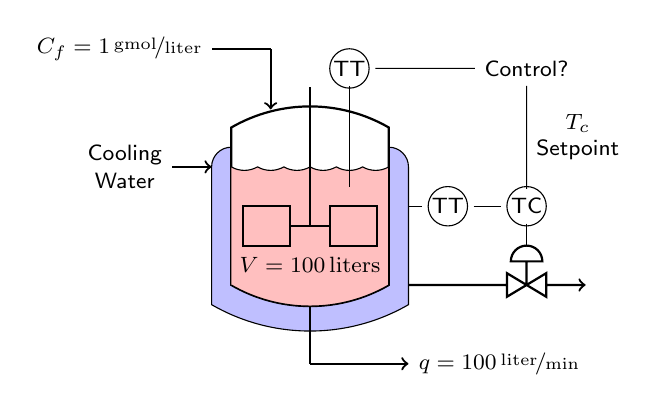
\begin{tikzpicture}
  %\draw[step=1cm,gray,very thin] (-1,0) grid (7,6);
  
  % Coordinates
  \coordinate (drum) at (1.5,3.5);
  \coordinate (feed) at (0.5,3);
  
  % cooling jacket
  \draw[fill=blue!25] (drum) ++(0,0.25) arc (90:180:0.25cm) -- 
    ++(0,-1.75) arc(240:300:2.5cm) -- ++(0,1.75) arc(0:90:0.25cm);

  \draw[thick,fill=white!100] (drum) --++(0,-1.5) arc (240:300:2cm)
    -- ++(0,2) arc (60:120:2cm) -- ++(0,-1);

  % Drum outline. Given location of the feed port, draws a drum with
  % stubs for the liquid and vapor lines located at ++(1,2) and ++(1,-2)
  \draw[fill=red!25] (drum) ++(0,-1.5) arc (240:300:2cm) -- ++(0,1.5)
    arc(-60:-120:0.333cm) arc(-60:-120:0.334cm) arc(-60:-120:0.333cm) 
    arc(-60:-120:0.333cm) arc(-60:-120:0.334cm) arc(-60:-120:0.333cm);
  \draw[thick, <-] (drum) ++(0.5,0.73) -- ++(0,0.77); 
  \draw[thick] (drum) ++(1,-1.768) --++ (0,-0.732);
  
  % Stirring paddle
  \draw [thick] (drum) ++ (1,-0.75) -- ++(-0.25,0) -- ++(0,0.25) 
    -- ++(-0.6,0) -- ++(0,-0.5) -- ++(0.6,0) -- ++(0,0.25) -- ++(0.25,0)
    -- ++(0.25,0) -- ++(0,0.25) -- ++(0.6,0) -- ++(0,-0.5) -- ++(-0.6,0)
    -- ++(0,0.25) -- ++(-0.25,0) -- ++(0,1.768);
    
  % Cooling lines
  \draw [thick,<-] (drum) ++(-0.25,0) -- ++ (-0.5,0) node[left] 
  	{\footnotesize \shortstack{Cooling\\ Water}};
  \draw [thick, ->] (drum) ++(2.25,-1.5) -- ++(1.25,0) ++ (0.25,0) 
    --++(0.25,0.15) --++(0,-0.3)
    --++(-0.5,0.3) --++(0,-0.3) --++(0.25,0.15) --++(0,0.3)
    --++(0.2,0) arc(0:180:0.2cm) --++(0.2,0) ++ (0.25,-0.3) -- ++(0.5,0);
  
  % Control elements
  \draw (drum) ++ (2.75,-0.5) circle (0.25cm) node (TT1) {\footnotesize TT};
  \draw (drum) ++ (3.75,-0.5) circle (0.25cm) node (TC1) {\footnotesize TC};
  \draw (drum) ++ (1.5,1.25) circle (0.25cm) node (TT2) {\footnotesize TT};
  \draw (TT2) ++ (2.25,0) node (control) {\footnotesize Control?};
  
  \draw (TT1) --++(-0.5,0);
  \draw (TT1) -- (TC1) --++ (0,-0.5);
  \draw (TT2) --++(0,-1.5);
  \draw (TT2) -- (control) -- (TC1) node[midway,right] 
  	{\footnotesize \shortstack{$T_c$ \\ Setpoint}};
   
  
  % connecting the units
  %\draw[->,thick] (feed) node [left] {$\dot{m}_1 = \unitfrac[4]{kg}{s}$} -- (drum);
  \draw[thick] (drum) ++ (0.5,1.5) -- ++(-0.75,0) 
    node [left] {\footnotesize $C_f = \unitfrac[1]{gmol}{liter}$};
  \draw[->,thick] (drum) ++ (1,-2.5) -- ++(1.25,0) 
    node [right] {\footnotesize $q = \unitfrac[100]{liter}{min}$};
  
  % label units
  \draw (drum) ++ (1,-1.25) node {\footnotesize $V = \unit[100]{liters}$};
  
\end{tikzpicture}
\end{document}